\documentclass{article}

\usepackage{amsmath, graphicx}

\graphicspath{ {./images/} }

\title{Ch. 27 HW \#1 Solutions}
\author{Principles of Macroeconomics}
\date{today}

\begin{document}

\maketitle

\section*{Quick Quiz}

\begin{enumerate}

\setcounter{enumi}{5}

\item (b) -- An increase in saving is an increase in supply. When the supply of loanable funds shifts right, the interest rate falls.

	\begin{center}
	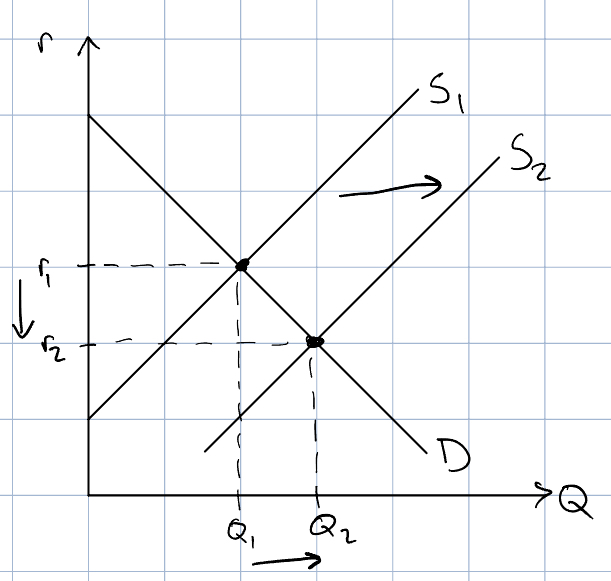
\includegraphics[width = 0.5\textwidth]{qq6}
	\end{center}

\item (c) -- If businesses expect capital to be more profitable, they will want to invest more. That increases their demand for loanable funds, so demand shifts right, and the interest rate rises. 

	\begin{center}
	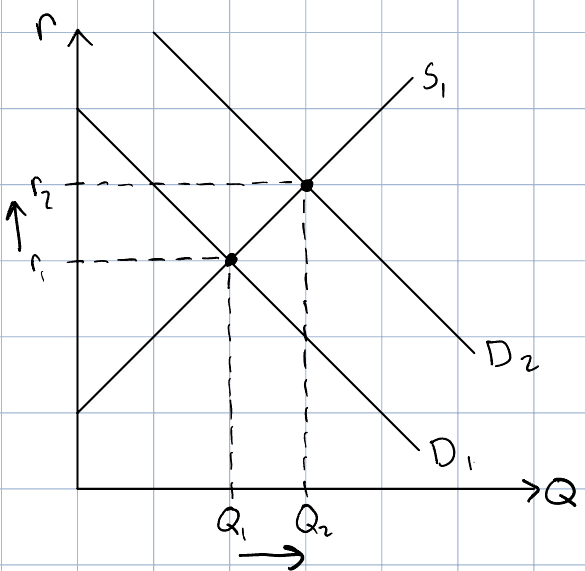
\includegraphics[width = 0.5\textwidth]{qq7}
	\end{center}

\item (b) -- An increase in the government budget deficit decreases public saving. That shifts the supply of loanable funds to the left, increases the interest rate, and decreases the equilibrium quantity of investment. That's why we say the government ``crowds out" investment when it runs a deficit.

	\begin{center}
	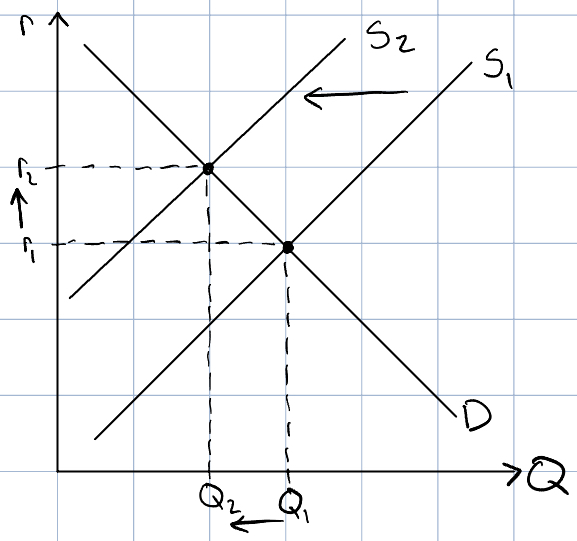
\includegraphics[width = 0.5\textwidth]{qfr6}
	\end{center}
	
\end{enumerate}




\section*{Questions for Review}

\begin{enumerate}

\setcounter{enumi}{2}

\item National saving is the total income left over after consumption and government purchases: $S_{Nat} = Y - C - G$ \\
	Private saving is the total income left over after consumption and taxes: $S_{Priv} = Y - T - C$ \\
	Public saving is the tax revenue left over after government purchases: $S_{Pub} = T - G$ \\
	National saving is the sum of private saving and public saving: \\ $S_{Nat} = S_{Priv} + S_{Pub}$
	
\item Investment is spending on capital goods. In a closed economy, investment equals national saving: $I = S_{Nat}$

\end{enumerate}



\section*{Problems and Applications}

\begin{enumerate}

\setcounter{enumi}{4}

\item \begin{gather*}
	S_{Priv} = Y - T - C = 10,000 - 1,500 - 6,000 = 2,500 \\
	S_{Pub} = T - G = 1,500 - 1,700 = -200 \\
	S_{Nat} = S_{Priv} + S_{Pub} = 2,500 - 200 = 2,300 \\
	I = S_{Nat} = 2,300
	\end{gather*}
	\begin{align*}
	I &= 3,300 - 100r \\
	2,300 &= 3,300 - 100r \\
	100r &= 1,000 \\
	r &= 10\%
	\end{align*}
	
\item

	\begin{enumerate}
	
	\item Higher interest rates make it more expensive for Intel to borrow money for the factory. That makes them less likely to build the factory. 
	
	\item It would. Higher interest rates make it more lucrative for Intel to save its money rather than spend it. That makes them more likely to save and less likely to build the factory.
	
	\end{enumerate}

\end{enumerate}

\end{document}